%%
%% This is file `sample-acmtog.tex',
%% generated with the docstrip utility.
%%
%% The original source files were:
%%
%% samples.dtx  (with options: `all,journal,bibtex,acmtog')
%% 
%% IMPORTANT NOTICE:
%% 
%% For the copyright see the source file.
%% 
%% Any modified versions of this file must be renamed
%% with new filenames distinct from sample-acmtog.tex.
%% 
%% For distribution of the original source see the terms
%% for copying and modification in the file samples.dtx.
%% 
%% This generated file may be distributed as long as the
%% original source files, as listed above, are part of the
%% same distribution. (The sources need not necessarily be
%% in the same archive or directory.)
%%
%%
%% Commands for TeXCount
%TC:macro \cite [option:text,text]
%TC:macro \citep [option:text,text]
%TC:macro \citet [option:text,text]
%TC:envir table 0 1
%TC:envir table* 0 1
%TC:envir tabular [ignore] word
%TC:envir displaymath 0 word
%TC:envir math 0 word
%TC:envir comment 0 0
%%
%% The first command in your LaTeX source must be the \documentclass
%% command.
%%
%% For submission and review of your manuscript please change the
%% command to \documentclass[manuscript, screen, review]{acmart}.
%%
%% When submitting camera ready or to TAPS, please change the command
%% to \documentclass[sigconf]{acmart} or whichever template is required
%% for your publication.
%%
%%
\documentclass[sigconf, noacm]{acmart}
\acmConference{\vphantom{}}{}{} % Suppresses the hanging commas

%%
%% \BibTeX command to typeset BibTeX logo in the docs
\AtBeginDocument{%
  \providecommand\BibTeX{{%
    Bib\TeX}}}

%% Rights management information.  This information is sent to you
%% when you complete the rights form.  These commands have SAMPLE
%% values in them; it is your responsibility as an author to replace
%% the commands and values with those provided to you when you
%% complete the rights form.


%%
%% Submission ID.
%% Use this when submitting an article to a sponsored event. You'll
%% receive a unique submission ID from the organizers
%% of the event, and this ID should be used as the parameter to this command.
%%\acmSubmissionID{123-A56-BU3}

%%
%% For managing citations, it is recommended to use bibliography
%% files in BibTeX format.
%%
%% You can then either use BibTeX with the ACM-Reference-Format style,
%% or BibLaTeX with the acmnumeric or acmauthoryear sytles, that include
%% support for advanced citation of software artefact from the
%% biblatex-software package, also separately available on CTAN.
%%
%% Look at the sample-*-biblatex.tex files for templates showcasing
%% the biblatex styles.
%%

%%
%% The majority of ACM publications use numbered citations and
%% references.  The command \citestyle{authoryear} switches to the
%% "author year" style.
%%
%% If you are preparing content for an event
%% sponsored by ACM SIGGRAPH, you must use the "author year" style of
%% citations and references.
\citestyle{acmauthoryear}

\setcopyright{none}
\pagestyle{plain}
\makeatletter
\let\@authorsaddresses\@empty
\makeatother
\acmVolume{}
\acmNumber{}
\acmArticle{}
\acmYear{}
\acmMonth{}
\acmBooktitle{}
\acmISBN{}
\acmDOI{}
\settopmatter{printacmref=false, printccs=false, printfolios=false}
\renewcommand\footnotetextcopyrightpermission[1]{}

%%
%% end of the preamble, start of the body of the document source.
\begin{document}

%%
%% The "title" command has an optional parameter,
%% allowing the author to define a "short title" to be used in page headers.
\title{Classification and Segmentation for Wildfire Detection: Optimized Deep Learning for UAVs}

%%
%% The "author" command and its associated commands are used to define
%% the authors and their affiliations.
%% Of note is the shared affiliation of the first two authors, and the
%% "authornote" and "authornotemark" commands
%% used to denote shared contribution to the research.
\author{Mohsen Hosseini}
\email{mohsen.hosseini@ucalgary.ca}
\affiliation{%
  \institution{The University of Calgary}
  \city{Calgary}
  \country{Canada}
}

\author{Maryam Kermanshahani}
\email{maryam.kermanshahani@ucalgary.ca}
\affiliation{%
  \institution{The University of Calgary}
  \city{Calgary}
  \country{Canada}
}
\author{Zahra Safari}
\email{zar.safari@ucalgary.ca}
\affiliation{%
  \institution{The University of Calgary}
  \city{Calgary}
  \country{Canada}
}

%%
%% By default, the full list of authors will be used in the page
%% headers. Often, this list is too long, and will overlap
%% other information printed in the page headers. This command allows
%% the author to define a more concise list
%% of authors' names for this purpose.
% \renewcommand{\shortauthors}{Trovato et al.}

%%
%% The abstract is a short summary of the work to be presented in the
%% article.
\begin{abstract}
Wildfires are a worldwide natural disaster causing important economic damages and loss of lives. Experts predict that wildfires will increase in the coming years mainly due to climate change. Early detection and prediction of fire spread can help reduce affected areas and improve firefighting~\cite{Ghali2022}. Unmanned aerial vehicles (UAVs) are increasingly used in forest fire monitoring and detection thanks to their high mobility and ability to cover areas at different altitudes and locations with relatively lower cost~\cite{Jiao2019}.  However, they are still limited by challenging problems such as small fire size, background complexity, and image degradation~\cite{Ghali2022}.
The proposed system integrates classification and segmentation techniques to identify and locate wildfires in aerial imagery. Leveraging the FLAME dataset and employing lightweight architectures such as MobileNet, Efficient-Net, and U-Net++, our models are optimized for deployment on resource-constrained UAVs. Experimental results demonstrate that the proposed system achieves 89\% accuracy and an F1 score of 90.3\% for classification, along with 99.83\% accuracy for segmentation, surpassing existing benchmarks.

\end{abstract}

%%
%% Keywords. The author(s) should pick words that accurately describe
%% the work being presented. Separate the keywords with commas.
\keywords{Wildfire Detection, UAV, Deep Learning, Classification, Segmentation, MobileNet, U-Net++}


%%
%% This command processes the author and affiliation and title
%% information and builds the first part of the formatted document.


\maketitle
\pagestyle{plain} % removes running headers

\section{Introduction}
Wildfires, driven by climatic changes, are becoming increasingly frequent and severe, leading to significant environmental, economic, and societal losses. Early detection and suppression of forest fires are crucial to minimizing the destruction that the fires may cause due to their rapid convection propagation and long combustion cycles. Massive efforts have been put into monitoring, detecting, and rapidly extinguishing forest fires before they become too large [A survey on technologies for automatic forest fire monitoring, detection, and fighting using unmanned aerial vehicles and remote sensing techniques]. Current remote sensing approaches to forest fire monitoring and detection can be grouped into ground-based systems, manned aerial vehicle-based systems, and satellite-based systems~\cite{DenBreejen1998}. Ground measurements have limited surveillance ranges. Satellite systems are less flexible in path planning and technology updates, with some drawbacks. Unmanned aerial vehicles (UAVs) with computer vision-based remote sensing systems are an increasingly realistic option, providing rapid, mobile, and low-cost alternatives for monitoring, detecting, and even fighting forest fires~\cite{Yuan2015}.  Furthermore, fire detection and segmentation showed impressive progress thanks to the use of deep learning (DL) techniques. DL-based fire detection methods are used to detect the color of a wildfire and its geometrical features such as angle, shape, height, and width. Their results are used as inputs to the fire propagation models. Several researches have been done in this area. 
In one of the papers, a novel deep ensemble learning method was developed to detect and classify wildfires using aerial images, which had impressive results~\cite{Ghali2022}. However, deploying deep learning models on UAVs presents unique challenges, including limited computational resources and the need for robust performance on small datasets.
By prioritizing efficient data use and reduced computational demands, our project aims to make wildfire detection more accessible to diverse operational settings. This issue is particularly relevant to our Deep Learning for Vision course, as it leverages machine learning techniques within the field of computer vision. In this project, we developed a system that combines classification and segmentation techniques to detect and localize wildfires from UAV imagery. Classification determines the presence of fire, while segmentation identifies the affected regions. This dual approach enhances detection accuracy and provides actionable insights for firefighting operations. By leveraging lightweight and efficient architectures, our system is tailored for real-world UAV deployments.


\section{Materials and Model Architecture (Visual representation of the model architecture)}
To achieve the objectives of wildfire detection, we explored various deep learning architectures optimized for classification and segmentation tasks. The selection of models and architectural enhancements are detailed below.

\subsection{Classification Model}

For the classification task, we experimented with both individual and ensemble models. 
\begin{itemize}
    \item Individual Models: MobileNet V3 (Small and Large), EfficientNet (B0, B3, B6), and ResNet (18, 34, 50). These models were chosen for their balance of computational efficiency and performance.
\end{itemize}
\begin{itemize}
    \item Ensemble Models: Combining two MobileNet models didn’t help. Therefore, we combined MobileNet V3 Large and EfficientNet B0, which gave the best results.
\end{itemize}
Therefore, we just chose MobileNet V3 Large with EfficientNet B0 as our model. Features extracted from both models were concatenated and passed through a fully connected layer for final classification. This ensemble leveraged the strengths of both architectures, improving detection accuracy. Figure~\ref{fig:architecture}  shows Our final network architecture for the classification.

\begin{figure}[h]
  \centering
  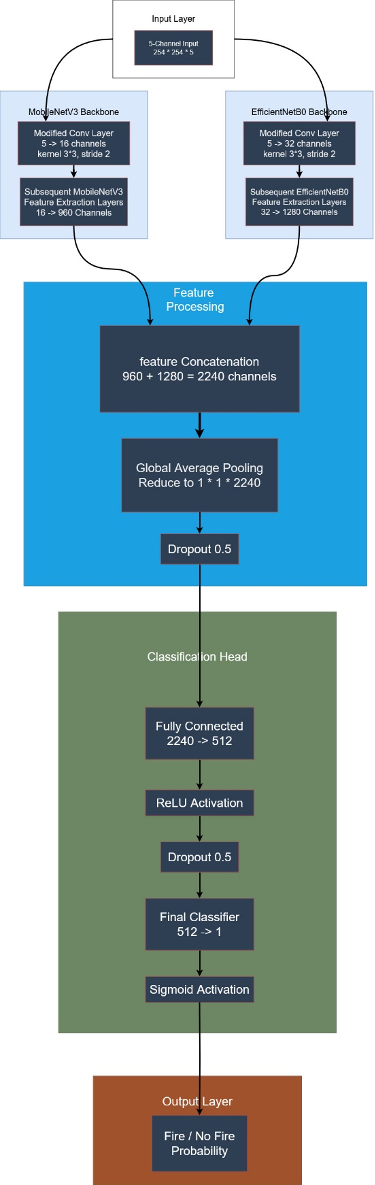
\includegraphics[width=\linewidth, height=0.8\textheight, keepaspectratio]{image_1}
  \caption{Classification network architecture.}
  \Description{Classification network architecture}
    \label{fig:architecture}
\end{figure}


\subsection{Segmentation Model}

For segmentation, we employed the U-Net++ architecture. In one of the previous works in this area, the U-net was used for a segmentation task. U-Net is a full convolution neural network for image semantic segmentation. Consists of encoder and decoder parts connected with skip connections. The encoder extracts features of different spatial resolutions (skip connections) which are used by the decoder to define an accurate segmentation mask~\cite{UNetModels}.
U-Net++, is similar to U-Net except that the decoder of U-Net++ is more complex than in usual U-Net~\cite{UNetModels}. U-Net++ was chosen for its convolutional design and efficiency compared to transformers. As for the encoder, we tried different encoders including MobileNet V3, ResNet (34, 101), and EfficientNet (B0, B6). None of them outperformed Regnet as the encoder. Figure ~\ref{fig:U-Net} shows the U-Net++ network architecture. 

\begin{figure}[h]
  \centering
  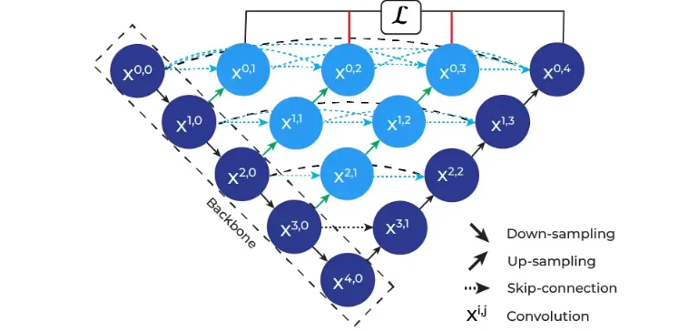
\includegraphics[width=\linewidth, keepaspectratio]{image_2}
  \caption{U-Net++ network architecture~\cite{UNetGFG}}
  \Description{U-Net++ network architecture}
    \label{fig:U-Net}
\end{figure}


\section{Dataset}

We used the FLAME dataset, a publicly available UAV-captured aerial imagery dataset designed for wildfire detection~\cite{FLAMEDataset}. This dataset contains labeled images with fire and no-fire categories and annotated segmentation masks for fire regions. However, there are some special points regarding working with our dataset in the classification and segmentation that we want to mention.

\subsection{Classification Data Preprocessing}

\textbf{Dataset Handling }
\begin{itemize}
    \item The dataset was not balanced, with having more fire samples than non-fire. Therefore, we used weighted sampling to balance the counts effectively for the model.
\end{itemize}
\begin{itemize}
    \item We had separated sources of Training and Test data. All other previous papers had performed their evaluation on this same test dataset. Therefore, we can compare our results with other papers, as our test data is identical. However, we did not have a validation set, as we did not have enough data, and we had the problem of overfitting. Therefore, we used part of our test data as the validation set. It was better not to use part of the test set as the validation set, but due to the overfitting problem and not having enough data, we did not have any other alternative option.
\end{itemize}

\textbf{Data Augmentation and Transforms }
\begin{itemize}
    \item Implement a Highlighter Red filter to mark fire areas. The results are shown in Figure ~\ref{fig:class-pre} for non-fire and fire images.
\end{itemize}
\begin{itemize}
    \item Apply Subel Filter to detect edges and distinguish between forest and random scenes
\end{itemize}
\begin{itemize}
    \item Utilize data augmentation techniques to increase model generalizability
\end{itemize}


\begin{figure}[h]
  \centering
  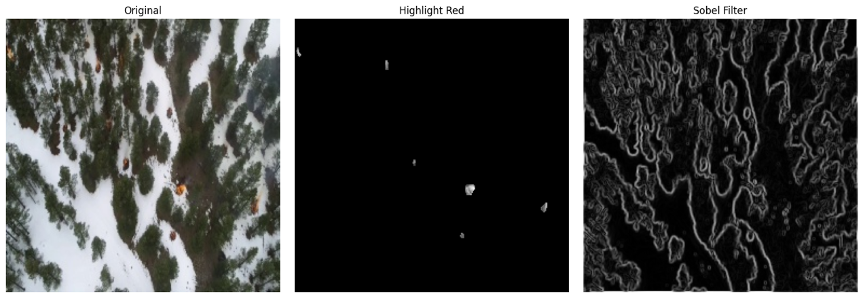
\includegraphics[width=\linewidth, keepaspectratio]{image_3}
  \caption{Classification preprocessing}
  \Description{Classification preprocessing}
  \label{fig:class-pre}
\end{figure}

\subsection{Segmentation Data}

\textbf{Dataset Handling }
\begin{itemize}
    \item Data was split into training, validation, and test sets based on a referenced paper. Our model did not see a test set and validation set at all.
\end{itemize}
\begin{itemize}
    \item Shuffling was avoided during testing to keep results consistent (However, during the training procedure we did the shuffling.)
\end{itemize}
\textbf{Data Augmentation and Transforms }
\begin{itemize}
    \item Apply Highlighter Red to mark fire regions and use Subel Filter to detect fire boundaries. The results of applying them can be seen in Figure~\ref{fig:pre}.
\end{itemize}


\begin{figure}[h]
  \centering
  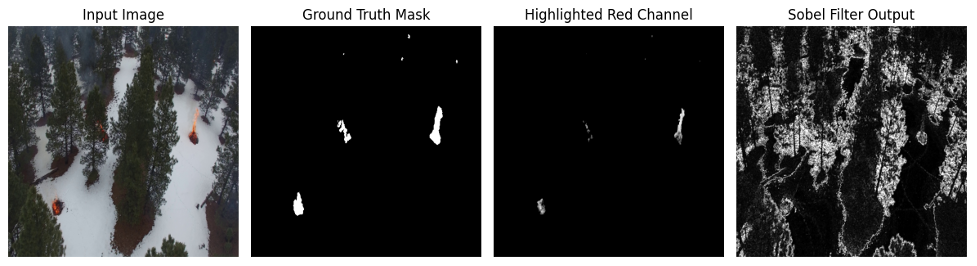
\includegraphics[width=\linewidth, keepaspectratio]{image_4}
  \caption{Classification preprocessing}
  \label{fig:pre}
  \Description{Classification preprocessing}
\end{figure}


\begin{itemize}
    \item Original image resolution of 4K (3800x2160) was too large for GPUs. Therefore, resolution was reduced to 512x512, which affected comparability with higher-resolution models.
\end{itemize}


\section{Training Procedure}

\subsection{Framework and Configuration}
All models were trained using the PyTorch framework with CUDA acceleration to leverage GPU processing power. We employed the Adam optimizer with an adaptive learning rate and used dropout and early stopping to prevent overfitting.

\subsection{Hardware Configuration}
\begin{itemize}
    \item GPU: Nvidia RTX 3080Ti
    \item RAM: 32 GB DDR4
    \item CPU: AMD Ryzen 9 5900X
    \item OS: Ubuntu 22.04
\end{itemize}

\subsection{Software and Frameworks}
\begin{itemize}
    \item Python version: 3.10.14
    \item Deep Learning Framework
    \begin{itemize}
        \item PyTorch version: 2.4.1
    \end{itemize}
    \begin{itemize}
        \item Torchvision for model architectures
    \end{itemize}
\end{itemize}

\subsection{Optimization Strategy}
\textbf{Classification Model}
1.	Optimization
\begin{itemize}
    \item Optimizer: We used AdamW as the optimizer. We also tried SGD, but AdamW was better. The reason why we used Adam was because we had the problem of overfitting. Results showed that Adam version with weight decay (short: AdamW) generalizes substantially better than Adam with L2 regularization~\cite{Loshchilov2017}
    \item Scheduler: We have a scheduler that from the validation set understands that when it should decrease the learning rate (to have a smooth and not oscillated loss decrease).
    \item Early stopping: When we find that in the validation set, we do not see any other better results, it just stops the training.
\end{itemize}
2.	Hyperparameter Configuration 
\begin{itemize}
    \item Batch Size: 50
    \item Epochs: 100 with early stopping
    \item Learning Rate: 0.001 (initial)
    \item Weight decay: 1e-4
\end{itemize}
3.	Regularization methods:
\begin{itemize}
    \item Dropout: Two dropout layers with 0.5 rate.
    \item L2 regularization through weight decay
    \item Using AdamW as an optimizer, which will help in regularization.
    \item Early stopping used.
\end{itemize}
4.	Performance metrics:
Figure ~\ref{fig:loss-curve}  describes the Training and Validation loss curve for our classification model.


\begin{figure}[h]
  \centering
  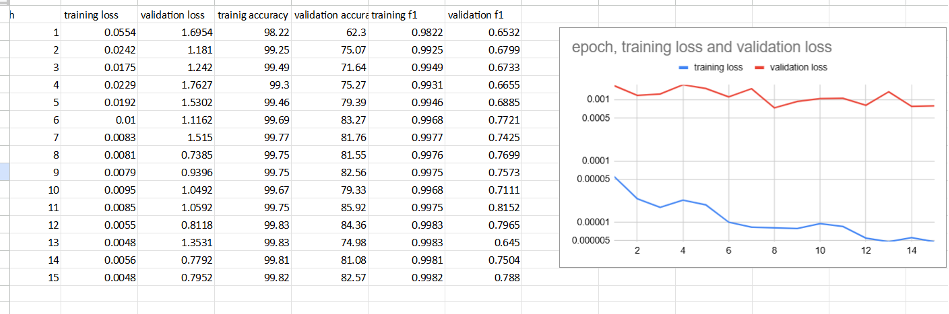
\includegraphics[width=\linewidth, keepaspectratio]{image_5}
  \caption{Classification training and validation loss curve}
  \Description{Classification training and validation loss curve}
  \label{fig:loss-curve}
\end{figure}

\textbf{Segmentation Model}

1.	Optimization 
\begin{itemize}
    \item Optimizer: Adam
    \item Scheduler: We have a scheduler that from the validation set understands when it should decrease the learning rate (to have a smooth and not oscillated loss decrease).
    \item Early stopping: When we find that in the validation set, we do not see any other better results, it just stops the training.
\end{itemize}
2.	Hyperparameter Configuration 
\begin{itemize}
    \item Batch Size: 4
    \item Epochs: 50 with early stopping
    \item Learning Rate with scheduler (initial): 1e-2
\end{itemize}
3.	Regularization methods:
\begin{itemize}
    \item L2 regularization
    \item Early stopping used.
\end{itemize}
4.	Performance metrics: 
Figure ~\ref{fig:lsegmentation-model} Training, Validation loss curve for our segmentation model. 

\begin{figure}[h]
  \centering
  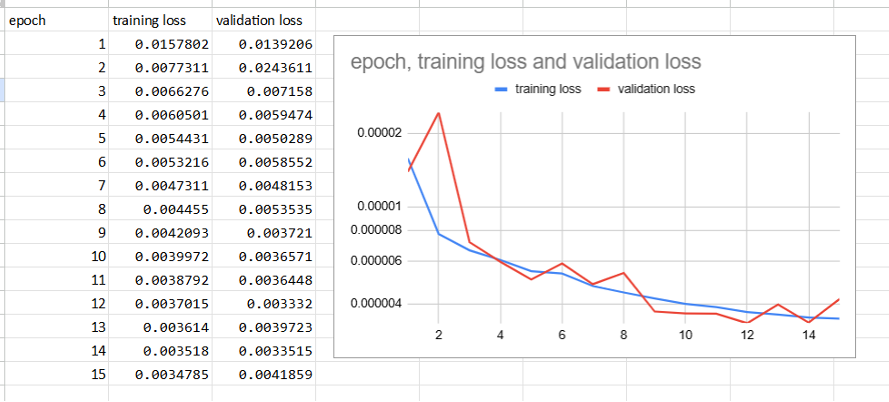
\includegraphics[width=\linewidth, keepaspectratio]{image_6}
  \caption{Segmentation training and validation loss curve}
  \Description{Segmentation training and validation loss curve}
  \label{fig:lsegmentation-model}
\end{figure}

\section{Evaluation Procedure}

The evaluation involved assessing the performance of both classification and segmentation models using established metrics. For classification, metrics such as accuracy, precision, recall, and F1 score were calculated to evaluate the detection of wildfire presence. Segmentation accuracy was assessed using mean F1 score, Intersection over Union (IoU), and mean recall, with a threshold of 0.6 for fire region detection.

\subsection {Classification}
Table ~\ref{tab:Classification} summarizes the performance of the proposed classification model compared to the reference model.

\begin{table} [h]
    \centering
    \begin{tabular}{ccc}
    \toprule
    Performance Metric & Our model & Reference model \\ % Column headings
    \midrule
    \ Overall accuracy & 88.95 & 85.12 \\ % Table rows
    \ Precision  & 86.24 (Fire: 95, No Fire: 82) & 94.20 \\
    \ Recall    & 94.76 (Fire: 86, No Fire: 93) & 83.10 \\
    \ F1 score   & 90.30 (Fire: 90, No Fire: 87) & 88.30 \\  
    \end{tabular}
    \caption{Classification test results}
    \label{tab:Classification}
\end{table}

Figure ~\ref{fig:confusion-matrix} is the classification confusion matrix that illustrates the performance of the proposed model. It shows strong results for both "Fire" and "No Fire" predictions, with minimal misclassifications.
Figure ~\ref{fig:Benchmark} is the benchmark confusion matrix that highlights the comparative performance. While the reference model achieved fewer false positives for "No Fire," it had a higher rate of false negatives for "Fire."

\begin{figure}[h]
  \centering
  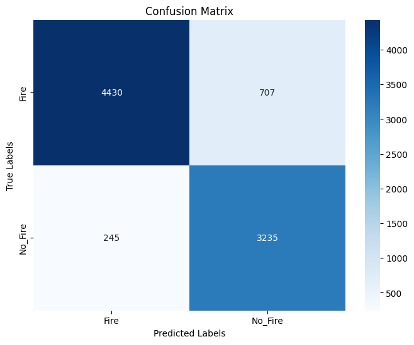
\includegraphics[width=\linewidth, keepaspectratio]{image_7}
  \caption{Classification confusion matrix}
  \Description{Classification confusion matrix}
    \label{fig:confusion-matrix}
\end{figure}



\begin{figure}[h]
  \centering
  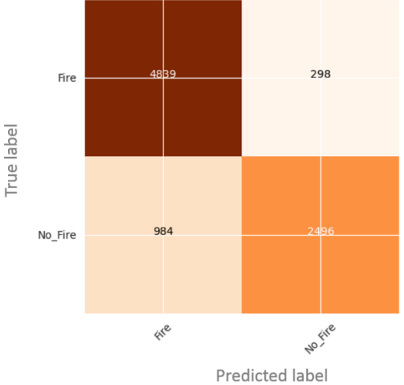
\includegraphics[width=\linewidth, keepaspectratio]{image_8}
  \caption{Benchmark confusion matrix}
  \Description{Benchmark confusion matrixBenchmark confusion matrix}
   \label{fig:Benchmark}
\end{figure}


\subsection {Segmentation}
For segmentation, Table ~\ref{tab:Segmentation} 
 Outline the results achieved using U-Net++ (our model), compared to the TransUNet-R50-ViT and U-Net models. A threshold of 0.6 was used for fire region detection.

\begin{table}[h]
    \centering
    \scriptsize % Reduce the font size of the table
    \begin{tabular}{p{4cm}c c c} % Use fixed-width columns
    \toprule
    Performance Metric & Our Model & TransUNet-R50-ViT Model & U-Net \\ % Column headings
    \midrule
    Mean F1 Score & 86.29 & 99.90 & 99.00 \\ % Corrected alignment
    Mean IoU & 75.96 & -- & -- \\ % Use '--' for empty cells
    Mean Accuracy (Macro) & 99.83 & 99.90 & 99.00 \\ 
    Mean Recall & 88.94 & -- & -- \\
    \bottomrule
    \end{tabular}
    \caption{Segmentation test results}
    \label{tab:Segmentation}
\end{table}


\section{Results}

Figure ~\ref{fig:fire-detection } shows the model prediction compared to the ground truth for a small fire in a snow-covered forest, demonstrating accurate fire region detection. Figure ~\ref{fig:detection-result} presents the model's performance for multiple small fire regions dispersed among trees, highlighting precise detection with slight under-segmentation in smaller areas.


\begin{figure}[h]
  \centering
  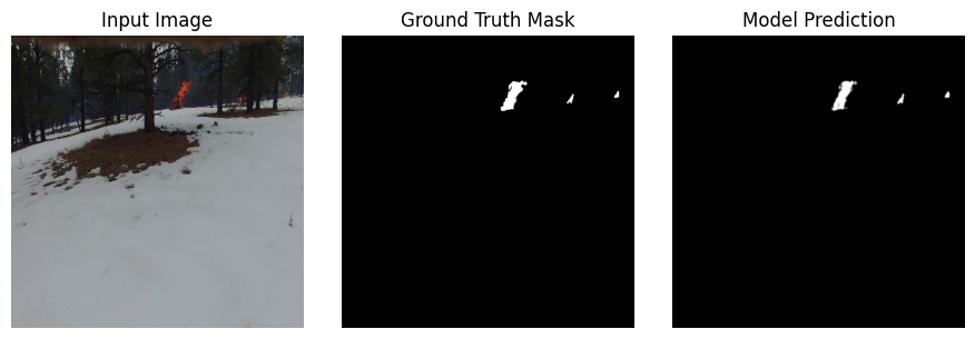
\includegraphics[width=\linewidth, keepaspectratio]{image_9}
  \caption{Model accurately detects fire regions in a snow-covered forest}
  \Description{Segmentation fire detection result}
  \label{fig:fire-detection }
\end{figure}


\begin{figure}[h]
  \centering
  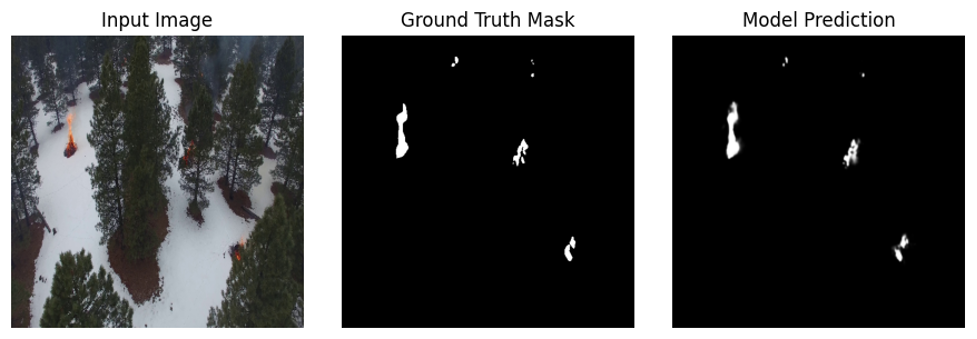
\includegraphics[width=\linewidth, keepaspectratio]{image_10}
  \caption{Model identifies multiple small fire regions among trees with minor under-segmentation.}
  \Description{Segmentation fire detection result}
  \label{fig:detection-result}
\end{figure}

\section{Discussion}
This study demonstrates the feasibility of deploying lightweight deep-learning models on UAVs for wildfire detection. The combination of classification and segmentation with performing proper preprocessing, and choosing proper models helped us to find promising results with much lighter models, and less hardware resources.

\textbf{Comparison with Related Work}
In terms of classification results, our model with 89\% accuracy outperformed our baseline paper by 85.12\%, with much lighter model. 
For the segmentation, with threshold = 0.6, we gained the maximum accuracy of 99.83, which was very close to the best benchmark result (99.99). However, our model is based on U-Net++ which is much lighter than transformer-based models, and needs less hardware resources. There were also some results in the benchmark for just using U-Net, but our model was better than that by 0.83. Moreover, our model is much lighter than a transformer-based network, which would make it a good option for using in UAVs.

\textbf{Future Work}
There are several directions for future works. Future research can work more on solving the overfitting problem. In addition, more data needs to be gathered, which may help to reduce the overfitting too. Another direction may use other types of architecture. For example, researchers can explore the integration of transformer-based models for improved segmentation accuracy.


\section{Conclusion}

This project successfully developed an efficient deep learning-based system for wildfire detection and localization using classification and segmentation. We gained a higher accuracy (89\%) compared with benchmark results (85\%), with a much lighter model. As for the segmentation, by threshold = 0.6, we gained the best accuracy (99.83\%) with U-Net++, which was very close to the best result for benchmark (99.9), which was with a transformer-based network. 
Our work had a focus on using preprocessing techniques. Our results show that how much preprocessing can be effective in wildfire classification. We used a lighter model, which was around 1/6 of the benchmark model, and we gained even better results. However, there are some challenges like overfitting problem, not enough data, that needs more work.

\bibliographystyle{ACM-Reference-Format} % Or any other style like plain, alpha, etc.
\bibliography{sample-base} % references.bib is the BibTeX file
\end{document}
\endinput
%%
%% End of file `sample-acmtog.tex'.
